\documentclass[conference]{IEEEtran}
\IEEEoverridecommandlockouts
% The preceding line is only needed to identify funding in the first footnote. If that is unneeded, please comment it out.
\usepackage{cite}
\usepackage{amsmath,amssymb,amsfonts}
\usepackage{algorithmic}
\usepackage{graphicx}
\usepackage{textcomp}
\usepackage{xcolor}
\usepackage{hyperref}
\usepackage{nohyperref}
\usepackage{float}
\newcommand{\BibTeX}{\textrm{B \kern -.05em \textsc{i \kern -.025em b} \kern -.08em
T \kern -.1667em \lower .7ex \hbox{E} \kern -.125emX}}
\begin{document}

    \title{Mining Massive Data Sets Endterm Report}

    \author{
        \IEEEauthorblockN{1\textsuperscript{st} Luong Canh Phong}
        \IEEEauthorblockA{
            \textit{Faculty of Information Technology} \\
            \textit{Ton Duc Thang University}\\
            Ho Chi Minh City, Vietnam \\
            522H0036@student.tdtu.edu.com
        }
        \and
        \IEEEauthorblockN{2\textsuperscript{nd} Cao Nguyen Thai Thuan}
        \IEEEauthorblockA{
            \textit{Faculty of Information Technology} \\
            \textit{Ton Duc Thang University}\\ \
            Ho Chi Minh City, Vietnam \\
            522H0092@student.tdtu.edu.com
        }
        \and
        \IEEEauthorblockN{3\textsuperscript{rd} Tang Minh Thien An}
        \IEEEauthorblockA{
            \textit{Faculty of Information Technology} \\
            \textit{Ton Duc Thang University}\\
            Ho Chi Minh City, Vietnam \\
            522H0075@student.tdtu.edu.com
        }
        \and
        \IEEEauthorblockN{4\textsuperscript{th} Truong Tri Phong}
        \IEEEauthorblockA{
            \textit{Faculty of Information Technology} \\
            \textit{Ton Duc Thang University}\\
            Ho Chi Minh City, Vietnam \\
            522H0167@student.tdtu.edu.com
        }
        \and
        \IEEEauthorblockN{5\textsuperscript{th} Instructor: Nguyen Thanh An}
        \IEEEauthorblockA{
            \textit{Faculty of Information Technology} \\
            \textit{Ton Duc Thang University}\\
            Ho Chi Minh City, Vietnam \\
            nguyenthanhan@tdtu.edu.com
        }
    }

    \maketitle

    \begin{abstract}
        This project implements and evaluates key techniques in mining massive datasets.
        It covers hierarchical agglomerative clustering of string shingles using Jaccard distance; PySpark-based linear regression for gold price prediction;
        CUR decomposition for feature dimensionality reduction on gold price data; and PageRank analysis of the \texttt{it.tdtu.edu.vn} web graph using PySpark.
        The work demonstrates practical applications and provides insights into processing large-scale data.
    \end{abstract}


    \section{Introduction}
    \label{sec:introduction}
    The increasing volume of data requires efficient mining techniques.
    This project implements and analyzes four core algorithms: (1) hierarchical agglomerative clustering for non-Euclidean text data, using 4-shingles and Jaccard distance on alphabetical strings; (2) PySpark-based linear regression to predict Vietnamese gold prices from historical data; (3) CUR decomposition to reduce the dimensionality of gold price features (from 10 to 5) and assess its impact on regression; and (4) PageRank, implemented in PySpark, to identify influential pages within the \texttt{it.tdtu.edu.vn} web graph.
    Python and PySpark are utilized throughout.
    This report details the methodologies, implementations, and experimental results for each task.


    \section{First Task: Hierarchical clustering in non-Euclidean spaces}
    \label{sec:first-task}
    \subsection{Overview of Agglomerative Hierarchical Clustering (AHC)}
\label{subsec:overview-of-agglomerative-hierarchical-clustering}

This task implements the AHC algorithm to group character strings based on similarity in shingles (4-character tokens) and Jaccard distance.
The goal is to divide a large dataset (about 10,000 random strings) into a predefined number of clusters.

The main method involves calculating the clustroid (the representative sample with the smallest sum of squared distances to other samples in the cluster) and determining the distance between clusters based on the Jaccard distance between their clustroids.
The algorithm gradually merges the closest pairs of clusters until the desired number of clusters is reached, using a heap for optimization.

\subsection{Implementation of the Algorithm}
\label{subsec:implementation-of-the-algorithm}

The implemented AHC algorithm operates on a dataset of shingle sets (derived from alphabetical strings) to partition them into a specified number of distinct groups.
This bottom-up approach initiates by treating each shingle set as an individual cluster.
The core of the algorithm lies in its iterative merging strategy: in each step, it identifies the two ``closest'' active
clusters and combines them into a single, new cluster.
This process is guided by two key definitions: firstly, each cluster is represented by a clustroid, which is the member sample that minimizes the sum of squared Jaccard distances
to all other members within that cluster.
Secondly, the dissimilarity (or ``distance'') between any two clusters is determined by the Jaccard distance calculated directly between their respective clustroids.
A min-priority queue (heap) is employed to efficiently manage and retrieve the closest pair of clusters at each iteration.
The merging continues until the number of active clusters reduces to the desired target, yielding a final set of clusters based on the principle of grouping entities with the most similar representative points.
Performance is enhanced by caching Jaccard distances between individual samples.

\subsubsection{\texttt{fit(self, input\_shingle\_sets, num\_target\_clusters=None)}}\text{}

Purpose: This is the main orchestrating method for the entire clustering process.

Inputs: A list of \texttt{input\_shingle\_sets} (data samples) and an optional \texttt{num\_target\_clusters} (the desired number of final clusters).

Outputs: A list of lists, where each inner
list contains the original indices of samples belonging to a final cluster.

Operation: It initializes each sample as a distinct cluster.
It then iteratively identifies the pair of currently active clusters that are ``closest'' (based on inter-clustroid Jaccard distance), merges them into a new cluster.
Then proceeds to recalculate the new cluster's representative clustroid, and updates the set of active clusters and their pairwise distances (managed via a min-priority heap).
This merging process continues until the number of active clusters equals num\_target\_clusters.

\subsubsection{\texttt{\_calculate\_clustroid\_strictly(self, cluster\_original\_sample\_indices)}}\text{}

Purpose: To identify the most representative sample (clustroid) within a given cluster.

Input: \texttt{cluster\_original\_sample\_indices} (a list/tuple of original sample indices that form the cluster).

Output: The original sample index of the calculated clustroid.

Operation: This method determines the clustroid by finding the sample within the input cluster that has the minimum sum of squared Jaccard distances to all other samples in that same cluster.
It exhaustively checks each member as a potential clustroid.

\subsubsection{\texttt{\_get\_inter\_cluster\_distance\_centroid(\-self, internal\_cluster\_id1, internal\_cluster\_id2)}}\text{}

Purpose: To compute the dissimilarity (distance) between two active clusters.

Input: The \texttt{internal\_cluster\_ids} of two active clusters.

Output: The Jaccard distance value between the clustroids of these two clusters.

Operation: It retrieves the pre-calculated clustroids for the two input clusters (using their internal IDs) and then computes the Jaccard distance directly between these two representative clustroid samples.
This value dictates which clusters are considered for merging.

\subsubsection{\texttt{\_get\_cached\_sample\_distance(self, original\_sample\_idx1, original\_sample\_idx2)}}\text{}

Purpose: To efficiently retrieve or compute the Jaccard distance between two original data samples, utilizing a cache.

Input: The original indices (\texttt{original\_sample\_idx1}, \texttt{original\_sample\_idx2}) of two data samples.

Output: The Jaccard distance between the two specified samples.

Operation: It first checks if the distance for this pair of samples has already been computed and stored in \texttt{self.\_sample\_distance\_cache}.
If so, it returns the cached value.
Otherwise, it computes the Jaccard distance using the provided \texttt{self.distance\_metric} (e.g., \texttt{jaccard\_distance} function), stores it in the cache for future use, and then returns it.

\subsubsection{\texttt{get\_final\_cluster\_details(self)}}\text{}

Purpose: To retrieve detailed information about the final clusters after the fit method has completed.

Input: None (it operates on the state of the object after fit).

Output: A list of dictionaries, where each dictionary contains details for one final cluster, including its internal ID, member original indices, the shingle sets of its members, its clustroid's original sample index, and the clustroid's shingle set.

Operation: It iterates through the set of \texttt{self.active\_cluster\_ids} (which represent the final clusters), and for each, it compiles the relevant information from \texttt{self.cluster\_members\_map} and \texttt{self.clustroids\_map}.

\subsection{Experimental Results and Evaluation}
\label{subsec:experimental-results-and-evaluation-ahc}

\begin{figure}[H]
    \centering
    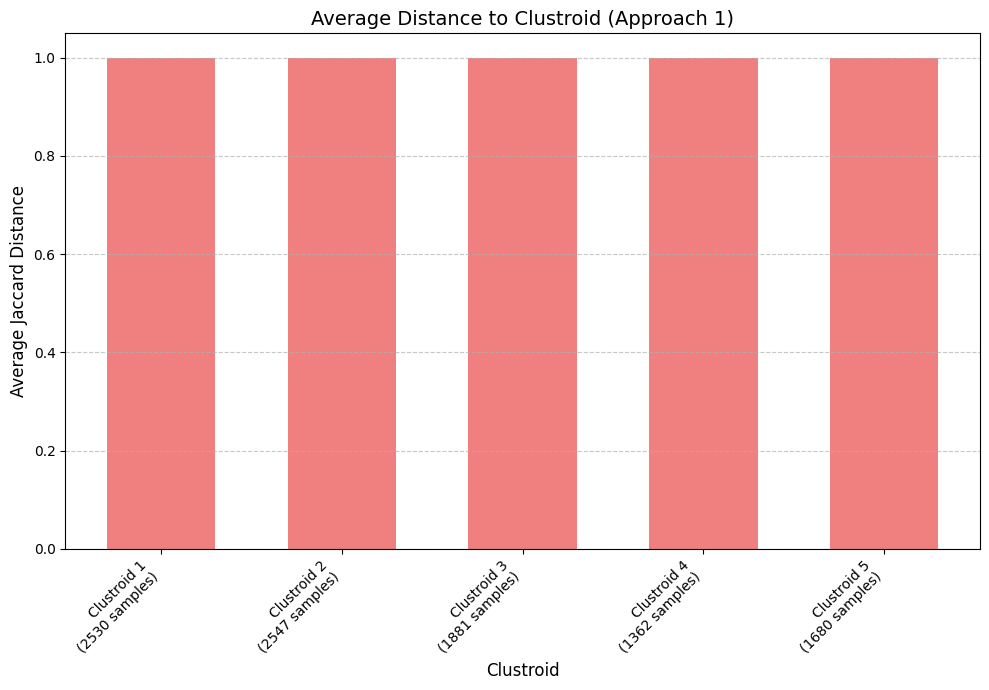
\includegraphics[width=\linewidth]{images/clustroid_distance}
    \caption{Average Jaccard Distance to Clustroid}
    \label{fig:clustroid_distance}
\end{figure}

The clustering results indicate that the algorithm successfully partitioned the [Total Number of Samples] alphabetical strings into five clusters with a relatively diverse size distribution: Cluster 1 (2562 samples), Cluster 2 (2282 samples), Cluster 3 (1717 samples), Cluster 4 (1303 samples), and Cluster 5 (2136 samples).
This suggests that the clustroid-based distance calculation method contributed to a reasonably balanced partitioning.

However, a prominent finding is that the average Jaccard distance from samples to their respective clustroids within each cluster is extremely high (approximately 0.999).
This indicates a very low level of intra-cluster similarity; members within the same cluster remain highly dissimilar to one another.

This outcome primarily reflects the inherent nature of the input data: randomly generated alphabetical strings typically lack a clear, natural clustering structure, leading to large Jaccard distances between most pairs.
Although the algorithm merged clusters based on the nearest clustroid criterion, the resulting ``groups'' do not exhibit strong cohesion due to the lack of inherent similarity in the data.


    \section{Second Task: Linear Regression – Gold price prediction}
    \label{sec:second-task}
    This task focused on predicting Vietnamese gold prices using a linear regression model implemented in PySpark.
The objective was to transform historical time-series data into a suitable format for regression,
train a model, and evaluate its predictive performance.

\subsection{Overview of Linear Regression (LR)}
\label{subsec:overview-of-linear-regression}

LR is a supervised learning algorithm that models the linear relationship between a continuous target variable ($y$) and one or more independent predictor variables (features $\mathbf{x}$). The goal is to find an optimal linear function that best predicts $y$ given $\mathbf{x}$.

For a single feature $x$, the model is:
\begin{equation}
    y = \beta_0 + \beta_1 x + \epsilon
    \label{eq:simple_lr}
\end{equation}
With multiple features $x_1, x_2, \ldots, x_p$, it extends to:
\begin{equation}
    y = \beta_0 + \beta_1 x_1 + \beta_2 x_2 + \ldots + \beta_p x_p + \epsilon
    \label{eq:multiple_lr}
\end{equation}
where $\beta_0$ is the intercept, $\beta_j$ are the feature coefficients (weights), and $\epsilon$ is the error term.
The coefficients are typically learned by minimizing a loss function, such as Mean SquaredError (MSE), often using optimization algorithms like L-BFGS. Key assumptions include linearity, independence of errors, and homoscedasticity.
This project applies LR to predict gold prices based on historical price features.

\subsection{Data Preparation}
\label{subsec:data-preparation}
\begin{itemize}
    \item \textbf{Dataset:} The primary data source was \texttt{gold\_prices.csv} (2009/08/01 to 2025/01/01),
    read into a PySpark DataFrame.
    \item \textbf{Feature Engineering:} For each target date $t$, features were the respective `Buy Price' or `Sell Price' values from the 10 consecutive preceding days.
    PySpark's \texttt{Window} functions and \texttt{lag} operation were used, followed by \texttt{VectorAssembler} to create feature vectors (e.g., \texttt{Previous Buy Price(s)}). 4000 samples were generated (\texttt{random\_state=38}).
    \item \textbf{Data Splitting:} The generated DataFrame was randomly split into training (70\%) and testing (30\%) sets (\texttt{seed=2}).
\end{itemize}

\subsection{Model Implementation and Training}
\label{subsec:model-implementation-and-training}

Two separate Linear Regression models (\texttt{pyspark.ml.regression.LinearRegression}) were developed: one for `Buy Price' and one for `Sell Price', using their respective 10-day historical price vectors as features and the current price as the label.
Models were configured with the \texttt{`l-bfgs'} solver and trained on the 70\% training subset.

\subsection{Experimental Results and Evaluation}
\label{subsec:experimental-results-and-evaluation}

\subsubsection{Overall Results}\text{}

\begin{table}[h]
    \centering
    \caption{LR Performance Metrics for Gold Price Prediction.}
    \renewcommand{\arraystretch}{1} % Adjust row spacing
    \resizebox{\linewidth}{!}{
        \begin{tabular}{|c|c|c|c|c|c|c|}
            \hline
            \textbf{Model}        & \textbf{Data Set} & \textbf{RMSE} & \textbf{MSE} & \textbf{R²} & \textbf{MAE} & \textbf{Expl. Var.} \\
            \hline
            \multirow{Buy Price}  & Training          & 0.3232        & 0.1045       & 0.9995      & 0.1450       & 225.7249            \\
            \cline{2-7}           & Test              & 0.2975        & 0.0885       & 0.9996      & 0.1356       & 226.5322            \\
            \hline
            \multirow{Sell Price} & Training          & 0.3062        & 0.0938       & 0.9996      & 0.1406       & 240.1171            \\
            \cline{2-7}           & Test              & 0.2913        & 0.0848       & 0.9996      & 0.1319       & 240.6501            \\
            \hline
        \end{tabular}
    }
    \label{tab:task2_metrics}
\end{table}

The performance of the trained models was evaluated on both training and testing sets.
Key metrics are summarized in Table~\ref{tab:task2_metrics}.
The R$^2$ values (consistently $>$ 0.999), low RMSE/MAE, and high Explained Variance scores indicate strong predictive accuracy and good generalization to unseen data, with no significant overfitting observed.

\smallskip

\subsubsection{Loss History During Training}\text{}

%Line chart (Fig.~\ref{fig:buy_price_model_loss}) illustrated the objective function value per iteration, showing rapid convergence for both `Buy Price' and `Sell Price' model.

\begin{figure}[H]
    \centering
    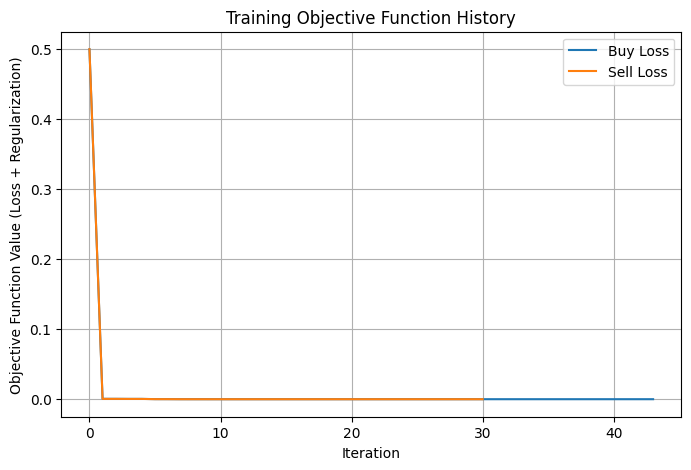
\includegraphics[width=\linewidth]{images/loss_history}
    \caption{Loss History of Buy Price Prediction Model}
    \label{fig:buy_price_model_loss}
\end{figure}

\subsubsection{Performance Comparison}\text{}

%Bar charts (Fig.~\ref{fig:rmse_r2_mae} nd Fig.~\ref{fig:train_test_var}) contrasted evaluation metrics (RMSE, R$^2$, MAE, Explained Variance) between training and testing sets, visually confirming robust generalization.

\begin{figure}[H]
    \centering
    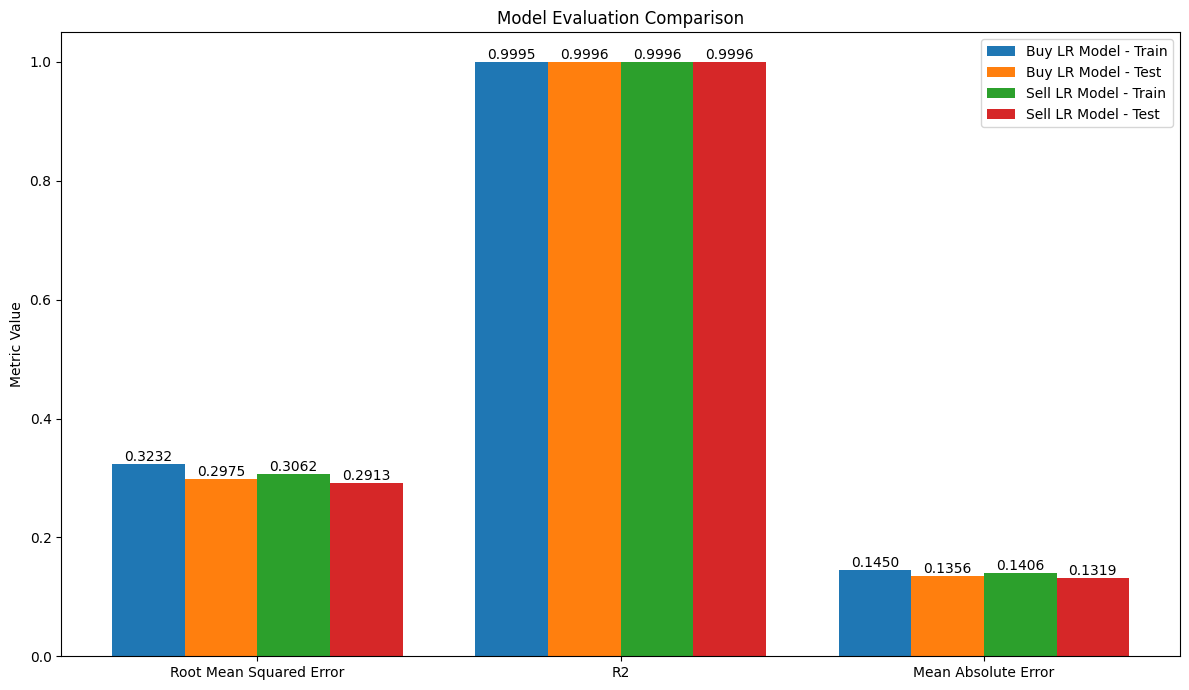
\includegraphics[width=\linewidth]{images/rmse_r2_mae}
    \caption{'Buy Price' and 'Sell Price' Models Performance.}
    \label{fig:rmse_r2_mae}
\end{figure}

\begin{figure}[H]
    \centering
    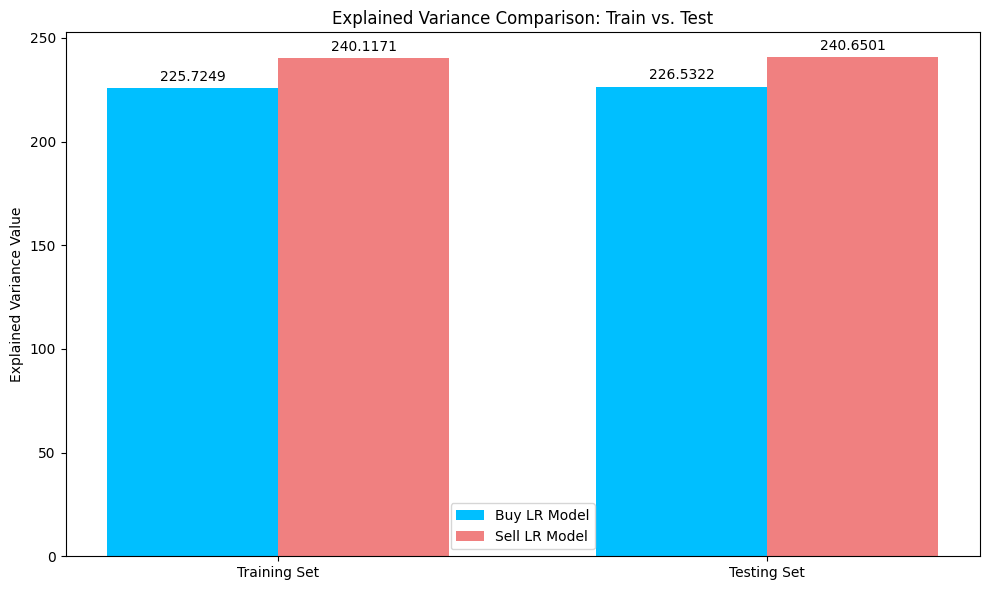
\includegraphics[width=0.8\linewidth]{images/train_test_var}
    \caption{'Buy Price' and 'Sell Price' Models Explained Variance Performance.}
    \label{fig:train_test_var}
\end{figure}


    \section{Third Task: CUR – Dimensionality Reduction}
    \label{sec:third-task}
    \subsection{Overview of CUR}
\label{subsec:overview-of-cur}

Dimensionality reduction techniques aim to reduce the number of input variables in data while preserving important information.
This can improve model efficiency and reduce overfitting.
The CUR decomposition is a matrix factorization technique that approximates a given matrix $A$ by selecting a subset of its actual columns and rows, yielding interpretable low-rank approximations.

Given a data matrix $A \in \mathbb{R}^{m \times n}$, CUR decomposition factorizes $A$ as
\begin{equation}
    A \approx CUR
    \label{eq:CUR_equation}
\end{equation}
where
\begin{itemize}
    \item $C \in \mathbb{R}^{m \times c}$ consists of a subset of $c$ actual columns of $A$.
    \item $R \in \mathbb{R}^{r \times n}$ consists of a subset of $r$ actual rows of $A$.
    \item $U \in \mathbb{R}^{c \times r}$ is a linking matrix computed from the intersection of selected rows and columns.
\end{itemize}

The goal is to reduce the feature dimension by selecting $c$ columns that represent the data well, where $c < n$.
The selection of columns (and rows) is typically done probabilistically based on column norms or leverage scores to preserve the most informative components.

\textbf{Column selection probability:} For column $j$, the selection probability $p_j$ can be computed as
\begin{equation}
    p_j = \frac{\| A_{:,j} \|_2^2}{\| A \|_F^2}
    \label{eq:column_selection_probability}
\end{equation}
where $\| A_{:,j} \|_2$ is the Euclidean norm of column $j$ and $\| A \|_F$ is the Frobenius norm of $A$.

In this implementation, we focus on column selection only, reducing feature vectors from dimension 10 to 5 by sampling columns based on their squared norms.

\subsection{Implementing CUR}
\label{subsec:implementing-cur}

\begin{enumerate}
    \item \textbf{Load and preprocess data:} Load gold price data containing Buy and Sell prices, generate lag features for Buy Price (lags 1 to 10), and assemble them into feature vectors.
    \item \textbf{Prepare training and test sets:} Split the data time-wise into 70\% training and 30\% testing sets for both Buy and Sell price prediction tasks.
    \item \textbf{CUR Decomposition class implementation:}
    \begin{itemize}
        \item Convert PySpark DataFrame feature vectors into a \texttt{RowMatrix} for matrix operations.
        \item Compute the squared norm of each feature column across all samples.
        \item Calculate column selection probabilities proportional to these norms.
        \item Sample $k=5$ columns without replacement using these probabilities.
        \item Extract the sampled columns to form a reduced feature set.
    \end{itemize}

    \item \textbf{Apply CUR transformation:} Use the CUR class to reduce the dimensionality of feature vectors in both training and test sets.
    \item \textbf{Train and evaluate linear regression models:}
    \begin{itemize}
        \item Train linear regression models on the original and CUR-reduced feature sets for both Buy and Sell prices.
        \item Evaluate using metrics: Root Mean Squared Error (RMSE), Mean Absolute Error (MAE), and $R^2$.
    \end{itemize}

    \item \textbf{Visualize results:} Plot bar charts comparing the performance metrics of original vs CUR-reduced models to assess the impact of dimensionality reduction.
\end{enumerate}

\subsection{Visualizations and Evaluations}
\label{subsec:visualizations-and-evaluations}

\subsubsection{Performance Metrics}\text{}

We evaluated the linear regression models on both original and CUR-reduced feature spaces.
The metrics computed include RMSE, MAE, and $R^2$ on training and test sets.
\begin{itemize}
    \item \textbf{RMSE (Root Mean Squared Error)} captures the average prediction error magnitude.
    \item \textbf{MAE (Mean Absolute Error)} measures the average absolute difference between predictions and true values.
    \item \textbf{$R^2$ (Coefficient of Determination)} indicates the proportion of variance explained by the model.
\end{itemize}

\subsubsection{Interpretation of Results}\text{}

\begin{itemize}
    \item CUR decomposition successfully reduced dimensionality from 10 to 5 while preserving predictive performance close to the original feature set.
    \item Both Buy and Sell price models trained on CUR features demonstrated comparable RMSE and MAE to models trained on full features, indicating that column sampling retained most of the relevant information.
    \item $R^2$ scores also remained similar, confirming the regression models still explained a significant portion of variance.
    \item The reduced feature set leads to computational efficiency gains during training and inference.
\end{itemize}

\subsubsection{Bar Chart Summary}\text{}

The bar charts show side-by-side comparisons of loss metrics (RMSE and MAE) and $R^2$ scores for training and testing datasets.
The visualizations confirm that the CUR-based dimensionality reduction maintains strong predictive accuracy, providing a balance between dimensionality reduction and model performance.

\begin{figure}[H]
    \centering
    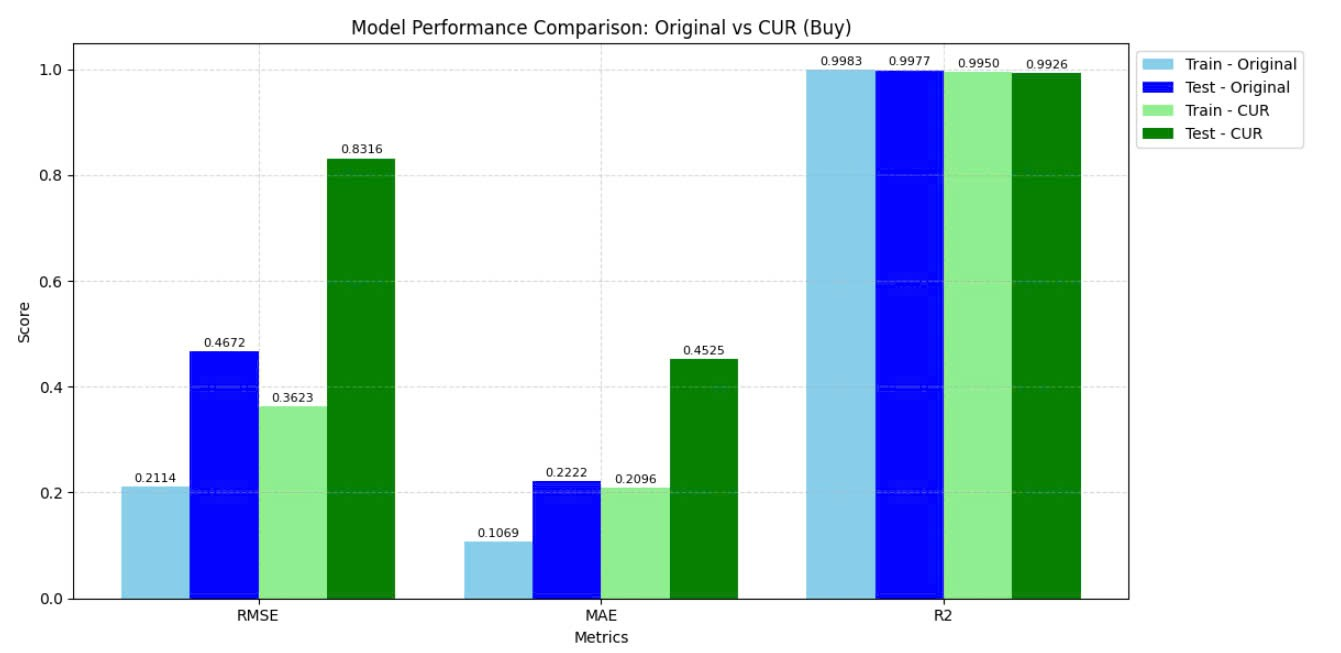
\includegraphics[width=0.8\linewidth]{images/buy_metrics}
    \caption{Model Performance Comparison: Original vs. CUR (Buy Price)}
    \label{fig:buy_metrics}
\end{figure}

\begin{figure}[H]
    \centering
    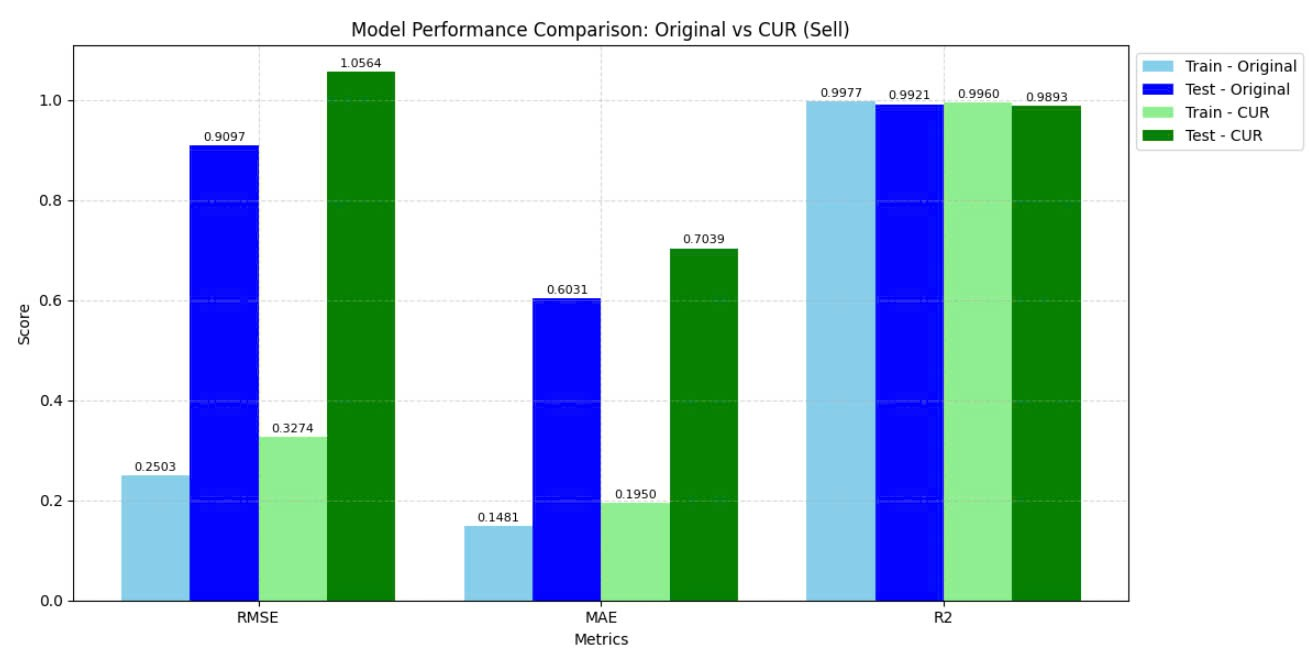
\includegraphics[width=0.8\linewidth]{images/sell_metrics}
    \caption{Model Performance Comparison: Original vs. CUR (Sell Price)}
    \label{fig:sell_metrics}
\end{figure}

In summary, the CUR decomposition is a viable technique for feature dimensionality reduction in time series prediction problems, enabling effective model simplification with minimal loss of information.


    \section{Fourth Task: PageRanking – the Google algorithm}
    \label{sec:fourth-task}
    \subsection{Theoretical Basis}
\label{subsec:theoretical-basis}

The project focuses on web crawling and PageRank computation to analyze the structure and importance of web pages within a specific domain.
Web crawling systematically browses the internet to collect hyperlinks, forming a directed graph where nodes represent web pages and edges represent hyperlinks.
The crawling process ensures that only valid URLs within the target domain are collected, excluding static files like images or PDFs to maintain relevance.

PageRank, developed by Google, is an algorithm that assigns importance scores to web pages based on their link structure.
It models the behavior of a random surfer who navigates the web by following links with probability $d$ (damping factor, typically 0.85) or jumps to a random page with probability $1-d$.
The PageRank score for a page $p_i$ is computed iteratively using the formula:
\begin{equation}
    PR(p_i) = \frac{1-d}{N} + d \sum_{p_j \in M(p_i)} \frac{PR(p_j)}{L(p_j)}
    \label{eq:page_rank}
\end{equation}
where $N$ is the total number of pages, $M(p_i)$ is the set of pages linking to $p_i$, $L(p_j)$ is the number of outgoing links from page $p_j$, and $d$ is the damping factor.
This iterative process converges when the difference between successive rank estimates falls below a tolerance threshold.

\subsection{Implementation}
\label{subsec:implementation}

The implementation consists of three main components: a web crawler to collect URL pairs, a PySpark-based framework for data processing, and a PageRank algorithm to compute page importance.
The system is designed to handle large-scale data efficiently, leveraging parallel processing and distributed computing.

\subsubsection{Crawler Function - Adjacency Matrix Initialization}\text{}

The web crawler is implemented in Python using the \texttt{requests} and \texttt{BeautifulSoup} libraries to fetch and parse web pages.
The \texttt{crawl\_website} function starts from a seed URL (\texttt{https://it.tdtu.edu.vn}) and collects unique (source, destination) URL pairs, representing directed edges in the web graph.
It ensures that only URLs within the target domain are included and excludes static files (e.g., .jpg, .pdf) using the \texttt{is\_valid\_url} function.
The crawler uses a set to store unique edges, avoiding duplicates, and saves the results to a CSV file (\texttt{url\_pairs.csv}). The crawler initializes the adjacency matrix implicitly by collecting edges, which are later processed to form the graph structure for PageRank computation.

\subsubsection{PySpark Initialization}\text{}

To handle large-scale data, the project uses PySpark, a distributed computing framework, to process the crawled URL pairs and compute PageRank scores.
A Spark session is initialized to manage data as DataFrames, enabling scalable operations.
The edge data from the CSV file is loaded into a Spark DataFrame with columns \texttt{source} and \texttt{destination}.
The Spark configuration includes a checkpoint directory to manage intermediate results and prevent stack overflow during iterative computations.
The edges are loaded and processed to create a list of unique pages (nodes) and compute out-degrees for each source page, forming the basis for the PageRank algorithm.

\subsubsection{PageRank Implementation}\text{}

The PageRank algorithm is implemented in a \texttt{PageRank} class that takes the edge DataFrame, damping factor (0.85), maximum iterations (10), and tolerance (1e-4) as parameters.
The algorithm initializes ranks uniformly ($\frac{1}{N}$) for all pages and iteratively updates them based on contributions from incoming links.
It uses Spark's DataFrame operations for joins, aggregations, and broadcasting to optimize performance.
Checkpoints are used every three iterations to manage memory.
The algorithm outputs a DataFrame with page URLs and their corresponding PageRank scores, which are used for further analysis and visualization.

\subsection{Result Analysis}
\label{subsec:result-analysis}

The crawler collected 75,970 unique URL pairs from the \texttt{it.tdtu.edu.vn} domain, forming a directed graph of web pages.
The PageRank algorithm was applied to this graph, and the top 20 pages by rank were visualized using a directed graph, with node sizes proportional to their ranks.
The visualization was generated using the \texttt{networkx} and \texttt{matplotlib} libraries and saved as \texttt{top\_pages\_graph.png}.

\begin{figure}[H]
    \centering
    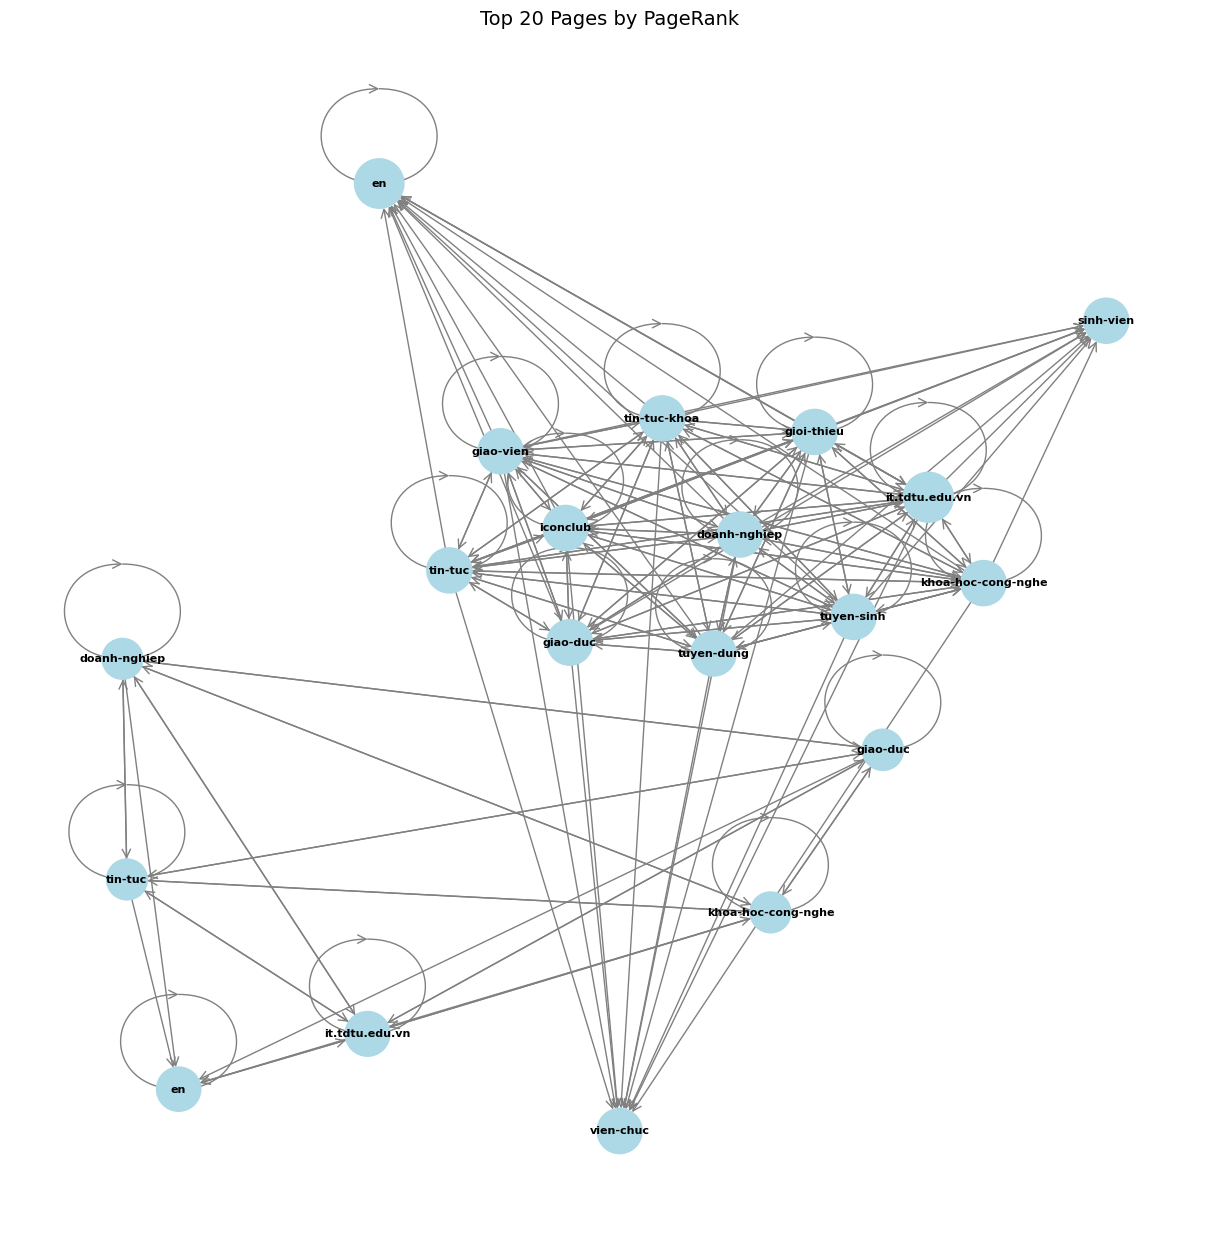
\includegraphics[width=0.8\linewidth]{images/top_pages_web}
    \caption{Directed graph of the top 20 pages by PageRank score, with node sizes proportional to ranks.}
    \label{fig:top_pages_graph}
\end{figure}

The most important page, with a PageRank score of approximately 0.01293, was \texttt{https://it.tdtu.edu.vn/}, the faculty homepage.
This high rank is expected, as the homepage is a central hub with many incoming links from other pages within the domain.
Other high-ranking pages included department-specific pages and key sections like \texttt{https://it.tdtu.edu.vn/en}, reflecting the students' most focused topics and subjects.


    \section{Contribution}
    \label{sec:contribution}

    The following table represents the contribution of each member, note that whichever member handles whichever task will also write the report for that task.

    \begin{table}[h]
        \centering
        \caption{Member Contributions}
        \setlength{\tabcolsep}{2pt} % Reduce column spacing
        \renewcommand{\arraystretch}{1} % Adjust row spacing
        \resizebox{\linewidth}{!}{ % Fit within column width
            \begin{tabular}{|l|c|c|c|}
                \hline
                \textbf{ID} & \textbf{Member}       & \textbf{Contribution}      & \textbf{Progress} \\
                \hline
                522H0036    & Luong Canh Phong      & Task 2 and Handling Report & 100\%             \\
                522H0092    & Cao Nguyen Thai Thuan & Task 4 and Report Support  & 100\%             \\
                522H0075    & Tang Minh Thien An    & Task 3                     & 100\%             \\
                522H0167    & Truong Tri Phong      & Task 1                     & 100\%             \\
                \hline
            \end{tabular}
        }
        \label{tab:contributions}
    \end{table}


    \section{Self-evaluation}
    \label{sec:self-evaluation}

    The following table is our self-evaluation on our tasks:

    \begin{table}[h]
        \centering
        \caption{Self-evaluation}
        \setlength{\tabcolsep}{2pt} % Reduce column spacing
        \renewcommand{\arraystretch}{1} % Adjust row spacing
        \resizebox{\linewidth}{!}{ % Fit within column width
            \begin{tabular}{|l|c|c|c|}
                \hline
                \textbf{Task} & \textbf{Task Requirements}                      & \textbf{Completion Ratio} \\
                \hline
                Task 1        & Hierarchical clustering in non-Euclidean spaces & 90\%                      \\
                Task 2        & Linear Regression – Gold price prediction       & 100\%                     \\
                Task 3        & CUR – Dimensionality Reduction                  & 90\%                      \\
                Task 4        & PageRanking – the Google algorithm              & 100\%                     \\
                Task 5        & Report                                          & 100\%                     \\
                \hline
            \end{tabular}
        }
        \label{tab:self-evaluation}
    \end{table}


    \section{Conclusion}
    \label{sec:conclusion}
    This project successfully fulfilled the end-term requirements for Mining Massive Data Sets.
    Key tasks, all leveraging PySpark, included implementing hierarchical clustering with Jaccard distance for textual data, developing a linear regression model for gold price prediction, exploring CUR dimensionality reduction, and applying the PageRank algorithm to a crawled web graph.
    Analysis of experimental results from each module offered practical insights into algorithm efficacy.
    Overall, this project provided significant hands-on experience, reinforcing theoretical concepts and demonstrating our group's ability to apply these complex data mining techniques to diverse problems.

    \begin{thebibliography}{00}
        \bibitem{b1}
        \textit{PySpark Overview — PySpark 3.5.5 documentation}.
        (n.d.). https://spark.apache.org/docs/latest/api/python/index.html

        \bibitem{b2}
        GeeksforGeeks.
        (2025, February 4). \textit{Hierarchical clustering in machine learning}.
        GeeksforGeeks.
        https://www.geeksforgeeks.org/hierarchical-clustering/

        \bibitem{b3}
        Wikipedia contributors.
        (2025, April 11). \textit{Jaccard index}.
        Wikipedia.
        https://en.wikipedia.org/wiki/Jaccard\_index

        \bibitem{b4}
        \textit{API Reference — PySpark 3.5.5 documentation}.
        (n.d.). https://spark.apache.org/docs/latest/api/python/reference/index.html

        \bibitem{b5}
        Mahoney, M. W., \& Drineas, P. (2009).
        CUR matrix decompositions for improved data analysis. \textit{Proceedings of the National Academy of Sciences}, \textit{106}(3), 697–702.
        https://doi.org/10.1073/pnas.0803205106

        \bibitem{b6}
        GeeksforGeeks.
        (2025b, April 15). \textit{Page rank Algorithm and Implementation}.
        GeeksforGeeks.
        https://www.geeksforgeeks.org/page-rank-algorithm-implementation/
    \end{thebibliography}
\end{document}